\documentclass[12pt,a4paper,UTF8]{ctexart}
\usepackage{graphicx}
\usepackage{amsmath}
\usepackage{amssymb}
\usepackage{cite}
\usepackage[ntheorem]{empheq}
\usepackage{enumitem}
\usepackage{fullpage}
\usepackage{tocbibind}
\usepackage[bookmarksopen=true,colorlinks,linkcolor=black]{hyperref}
\usepackage{cellspace}
\usepackage{listings}
\usepackage{color}
\usepackage{epstopdf}
\usepackage{subfigure}
\usepackage{algorithm}
\usepackage{algorithmicx}
\usepackage{algpseudocode}

\renewcommand{\algorithmicrequire}{\textbf{Input:}}  % Use Input in the format of Algorithm
\renewcommand{\algorithmicensure}{\textbf{Output:}} % Use Output in the format of Algorithm

\usepackage{longtable}

\usepackage{float}
\definecolor{gray}{rgb}{0.5,0.5,0.5}
\definecolor{dkgreen}{rgb}{.068,.578,.068}
\definecolor{dkpurple}{rgb}{.320,.064,.680}

% set Matlab styles
\lstset{
   language=Matlab,
   keywords={break,case,catch,continue,else,elseif,end,for,function,
      global,if,otherwise,persistent,return,switch,try,while},
   basicstyle=\ttfamily,
   keywordstyle=\color{blue}\bfseries,
   commentstyle=\color{dkgreen},
   stringstyle=\color{dkpurple},
   backgroundcolor=\color{white},
   tabsize=4,
   showspaces=false,
   showstringspaces=false
}

\begin{document}
\CJKfamily{zhkai}	


\begin{center}
\textbf{作业二}\\
\textbf{姓名\quad 徐家恒~~~~~~~~~~~~~ 学号 PB18000334~~~~~~~~~~~~~~ 日期 2021.	5.31}\\
\end{center}

\begin{center}
\fbox{
\begin{minipage}{40em}
\vspace{5cm}
\hspace{20cm}
\end{minipage}}
\end{center}
\vspace{1cm}

\begin{enumerate}
	\item[第一题]
	本题考虑对于定义在$[-1, 1]$上的一个光滑函数$f(x)$的三次样条插值的使用。下面所说的误差都是指绝对误差。

	(a) (10分)仿照课堂笔记或课本推导出关于额外给定边界点处(即-1和1)三次样条插值多项式的一次导数值时其在各插值点上的二次导值应该满足的线性方程组。请给出推导过程。\\

	在每个小区间$[x_i,x_{i+1}]$上做线性插值,假定已知$f^{\prime \prime}(x_i)=M_i$
	$$
		f^{\prime \prime}_i (x)=\frac{x-x_{i+1}}{x_i-x_{i+1}} M_i+\frac{x-x_{i}}{x_{i+1}-x_{i}} M_{i+1},x_i\leq x\leq x_{i+1}
	$$
	对$f^{\prime \prime}(x)$积分两次,记$h_i=x_{i+1}-x_i$
	$$
	\begin{aligned}
		f(x) &=  f_i(x) = \frac{(x-x_{i+1})^3}{6h_i}M_i+\frac{(x-x_i)^3}{6h_i}M_{i+1}+cx+d\\
			&=\frac{(x-x_{i+1})^3}{6h_i}M_i+\frac{(x-x_i)^3}{6h_i}M_{i+1}+C(x_{x+1}-x)+D(x-x_i)
	\end{aligned}
	$$
	将$f (x_i)=y_i,f (x_{i+1})=y_{i+1}$带入上式解出
	$$
		C=\frac {y_i} {h_i} - \frac {h_i M_i} {6}, D=\frac {y_{i+1} }{h_{i+1}} - \frac {h_{i+1} M_{i+1}} {6}
	$$
	$$
	\begin{aligned}
		f(x) &= \frac{(x_{i+1}-x)^3 M_i+(x-x_i)^3 M_{i+1}}{6h_i}+\frac{(x_{i+1}-x)^3 y_i+(x-x_i)^3 y_{i+1}}{6h_i}\\
		&- \frac{h_i}{6} [(x_{i+1}-x)M_i+(x-x_i)M_{i+1}],x\in [x_i,x_{i+1}]
	\end{aligned}
	$$
	在内节点$x_i$,由$f^\prime_i(x_i)=f^\prime_{i-1}(x_i)$可得到
	$$
		f(x_i,x_{i+1})-\frac{h_i}{3}M_i-\frac{h_i}{6}M_{i+1}=f(x_{i-1},x_{i})-\frac{h_{i-1}}{3}M_{i-1}-\frac{h_{i-1}}{6}M_{i}
	$$
	整理后得到
	$$
		\mu_i M_{i-1} +2M_i+\lambda_i M_{i+1} =d_i, i=1,2,\dots,n-1
	$$
	其中
	$$
		\lambda_i = \frac{h_i}{h_i+h_{i-1}},\mu_i = 1-\lambda_i
	$$
	$$
		d_i = \frac{6}{h_i+h_{i-1}}(\frac{y_{i+1}-y_i}{h_i}-\frac{y_i-y_{i-1}}{h_{i-1}})=6f(x_{i-1},x_i,x_{i+1})
	$$
	将$f^\prime(x_0)=m_0,f^\prime(x_n)=m_n$的值分别带入对应表达式,得
	$$
		2M_0+M_1=\frac{6}{h_0}[f[x_0,x_1]-m_0]=d_0
	$$
	$$
		M_{n-1}+2M_n=\frac{6}{h_n-1}[m_n-f[x_{n-1},x_n]]=d_n
	$$
	得到$n+1$个未知量,$n+1$个方程组
	$$
		\left[\begin{array}{llllll}
			2   & 1 &        &        &    &    \\
	        \mu_1  & 2  & \lambda_1     &        &    &    \\
           		& \mu_2 & 2      & \lambda_2 &    &    \\
            	&    & \ddots & \ddots & \ddots &    \\
            	&    &        & \mu_{n-1}     & 2  & \lambda_{n-1} \\
            	&    &        &        & 1 & 2
		\end{array}\right]
		\left[\begin{array}{l}
			M_0\\
			M_1\\
			M_2\\
			\vdots \\
			M_{n-1} \\
			M_n
		\end{array}\right]=
		\left[\begin{array}{l}
			d_0\\
			d_1\\
			d_2\\
			\vdots \\
			d_{n-1} \\
			d_n
		\end{array}\right]
	$$


	(b) (10分)令三次样条插值多项式在-1和1处的导数为0,用Matlab基于上一问中的结果使用n = 24个子区间插值一个定义$[-1, 1]$上的函数$f(x) =\sin(4x^2) + \sin^2(4x)$并使用semilogy图通过在2000个等距点上取真实值画出你构造的三次样条插值的逐点误差。\\

	代码:\\
\begin{lstlisting}[frame=single,numbers=left]
clc,close
syms x;
left = -1;
right = 1;
n = 2.^4;
n1 = 2000;
m0 = 0;
mn = 0;
step = (right - left)/n;
step1 = (right - left)/n1;
y = @(x) sin(4 * x.^2) + (sin(4 * x)).^2;
x2 = left:step1:right;
res = myFunc(y, left, right, n, m0, mn);
fy = zeros(1, n1 + 1);
dev = zeros(1, n1 + 1);
for i = 1 : n1
    seq = floor((x2(i) - left)/step) + 1;
    fy(i) = res(seq, 1) * x2(i).^3 + res(seq, 2) ...
	* x2(i).^2 + res(seq, 3) * x2(i) + res(seq, 4);
    dev(i) = abs(fy(i) - y(x2(i)));
end
figure
semilogy(x2, dev)

function [res] = myFunc(y, left, right, n, m0, mn)
    sym y;
    step = (right - left)/n;
    lambda = 1/2;
    mu = 1 - lambda;
    d = zeros(n + 1, 1);
    A = zeros(n + 1, n + 1);
    res = zeros(n, 4);
    para = left;
    for i = 2 : n
        para = para + step;
        d(i, 1) = 6 * (y(para + step) + y(para - step) ...
		 - 2 * y(para)) / (2 * step.^2);
        A(i, i - 1) = mu;
        A(i, i) = 2;
        A(i, i + 1) = lambda;
    end
    d(1, 1) = 6 / step * ((y(left + step) ...
	 - y(left))/step - m0);
    d(n + 1, 1) = 6 / step * (mn - (y(right) ...
	- y(right - step))/step);
    A(1, 1) =  2;
    A(1, 2) = 1;
    A(n + 1, n) = 1;
    A(n + 1, n + 1) = 2;
    m = A\d;
    
    para = left;
    for i = 1 : n
        para1 = para + step;
        A1 = [
            para.^3 para.^2 para 1;
            para1.^3 para1.^2 para1 1;
            6 * para 2 0 0;
            6 * para1 2 0 0;
            ];
        Y = [
            y(para);
            y(para1);
            m(i, 1);
            m(i + 1, 1);
            ];
        X = A1\Y;
        for j = 1 : 4
            res(i, j) = X(j, 1);
        end
        para = para1;
    end
end
\end{lstlisting}


	得到的逐点误差如下图\ref{jpg:1}\\
	\begin{figure}[H]
		\centering
     	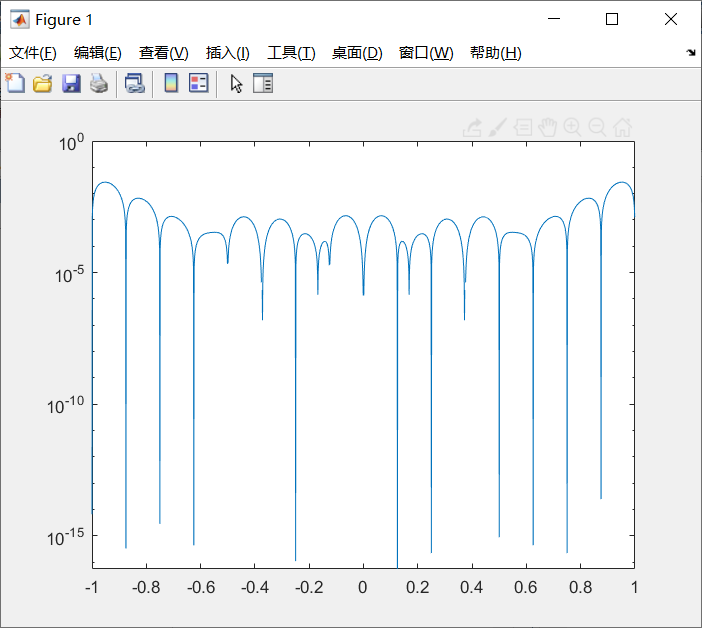
\includegraphics[width=0.8\textwidth]{1.png}
    	\caption{-1和1处导数为0的插值误差图像}\label{jpg:1}
	\end{figure}

	(c) (15分)使用不同的n,令$n = 2^4, 2^5, \dots, 2^10$重复上一问,取关于不同n的2000个等距点上的误差的最大值,用loglog图描述插值区间上最大误差值随n变化的情况(即横轴是n)。\\

	代码:\\
\begin{lstlisting}[frame=signle,numbers=left]
clc,close
syms x;
left = -1;
right = 1;
n1 = 2000;
m0 = 0;
mn = 0;
step1 = (right - left)/n1;
y = @(x) sin(4 * x.^2) + (sin(4 * x)).^2;
x1 = left:step1:right;

arr_n = [2.^4, 2.^5, 2.^6, 2.^7, 2.^8, 2.^9, 2.^10];
[~, ll] = size(arr_n);
maxn = zeros(1, ll);
figure
for j = 4 : 10
    n = 2.^j;
    step = (right - left)/n;
    x = left:step:right;
    res = myFunc(y, left, right, n, m0, mn);
    fy = zeros(1, n1 + 1);
    dev = zeros(1, n1 + 1);
    for i = 1 : n1
        seq = floor((x1(i) - left)/step) + 1;
        fy(i) = res(seq, 1) * x1(i).^3 + res(seq, 2) ...
		* x1(i).^2 + res(seq, 3) * x1(i) + res(seq, 4);
        dev(i) = abs(fy(i) - y(x1(i)));
    end
    maxn(j - 4 + 1) = max(dev(i));
end
loglog(arr_n, maxn)


function [res] = myFunc(y, left, right, n, m0, mn)
    sym y;
    step = (right - left)/n;
    lambda = 1/2;
    mu = 1 - lambda;
    d = zeros(n + 1, 1);
    A = zeros(n + 1, n + 1);
    res = zeros(n, 4);
    para = left;
    for i = 2 : n
        para = para + step;
        d(i, 1) = 6 * (y(para + step) + y(para - step)...
		 - 2 * y(para)) / (2 * step.^2);
        A(i, i - 1) = mu;
        A(i, i) = 2;
        A(i, i + 1) = lambda;
    end
    d(1, 1) = 6 / step * ((y(left + step)...
	 - y(left))/step - m0);
    d(n + 1, 1) = 6 / step * (mn - (y(right)...
	 - y(right - step))/step);
    A(1, 1) =  2;
    A(1, 2) = 1;
    A(n + 1, n) = 1;
    A(n + 1, n + 1) = 2;
    m = A\d;
    
    para = left;
    for i = 1 : n
        para1 = para + step;
        A1 = [
            para.^3 para.^2 para 1;
            para1.^3 para1.^2 para1 1;
            6 * para 2 0 0;
            6 * para1 2 0 0;
            ];
        Y = [
            y(para);
            y(para1);
            m(i, 1);
            m(i + 1, 1);
            ];
        X = A1\Y;
        for j = 1 : 4
            res(i, j) = X(j, 1);
        end
        para = para1;
    end
end
\end{lstlisting}

		得到的最误差如下图\ref{jpg:2}\\
	\begin{figure}[H]
		\centering
     	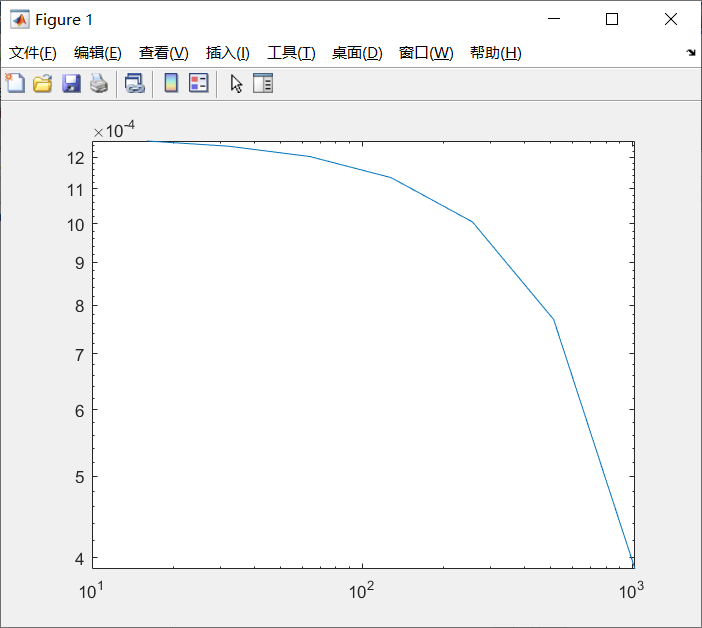
\includegraphics[width=0.8\textwidth]{2.png}
    	\caption{-1和1处导数为0时不同n值的最大误差图像}\label{jpg:2}
	\end{figure}

	(d) (15分)针对周期边界条件,即假设三次样条函数满足$S^{\prime }(-1) = S^{\prime}(1)和S^{\prime \prime}(−1) =S^{\prime \prime}(1)$,重复完成上面三问中的要求。\\

	此时边界关系变为$$S^{\prime }(-1) = S^{\prime}(1),S^{\prime \prime}(−1) =S^{\prime \prime}(1)$$
	即$$m_0=m_n,M_0=M_n$$
	则(a)中矩阵方程可以简化为
	
	$$
		\left[\begin{array}{llllll}
			4   & 1 &  1      &        &    &    \\
	        \mu_1  & 2  & \lambda_1     &        &    &    \\
           		& \mu_2 & 2      & \lambda_2 &    &    \\
            	&    & \ddots & \ddots & \ddots &    \\
            	&    &        & \mu_{n-2}     & 2  & \lambda_{n-2} \\
            \lambda_{n-1}	&    &        &        & \mu_{n-1} & 2
		\end{array}\right]
		\left[\begin{array}{l}
			M_0\\
			M_1\\
			M_2\\
			\vdots \\
			M_{n-2} \\
			M_{n-1}
		\end{array}\right]=
		\left[\begin{array}{l}
			d_0\\
			d_1\\
			d_2\\
			\vdots \\
			d_{n-2} \\
			d_{n-1}
		\end{array}\right]
	$$

	$n=2^4$计算逐点误差代码:\\
\begin{lstlisting}[frame=single,numbers=left]
clc,close
syms x;
left = -1;
right = 1;
n = 2.^4;
n1 = 2000;
m0 = 0;
mn = 0;
step = (right - left)/n;
step1 = (right - left)/n1;
y = @(x) sin(4 * x.^2) + (sin(4 * x)).^2;
x2 = left:step1:right;
res = myFunc(y, left, right, n);
fy = zeros(1, n1 + 1);
dev = zeros(1, n1 + 1);
for i = 1 : n1
    seq = floor((x2(i) - left)/step) + 1;
    fy(i) = res(seq, 1) * x2(i).^3 + res(seq, 2)...
	 * x2(i).^2 + res(seq, 3) * x2(i) + res(seq, 4);
    dev(i) = abs(fy(i) - y(x2(i)));
end
figure
semilogy(x2, dev)

function [res] = myFunc(y, left, right, n)
    sym y;
    step = (right - left)/n;
    lambda = 1/2;
    mu = 1 - lambda;
    d = zeros(n, 1);
    A = zeros(n, n);
    res = zeros(n, 4);
    para = left;
    for i = 2 : n
        para = para + step;
        d(i, 1) = 6 * (y(para + step) + y(para - step)...
		 - 2 * y(para)) / (2 * step.^2);
    end
    d(1, 1) = 6 / step * (y(left + step) - y(left)...
	 + y(right) - y(right - step)) / step;
    A(1, 1) =  4;
    A(1, 2) = 1;
    A(1, 3) = 1;
    for i = 2 : n - 1
        A(i, i - 1) = mu;
        A(i, i) = 2;
        A(i, i + 1) = lambda;
    end
    A(n, 1) = lambda;
    A(n, n - 1) = mu;
    A(n, n) = 2;
    m = A\d;
    m(n + 1, 1) = m(1, 1);
    para = left;
    for i = 1 : n
        para1 = para + step;
        A1 = [
            para.^3 para.^2 para 1;
            para1.^3 para1.^2 para1 1;
            6 * para 2 0 0;
            6 * para1 2 0 0;
            ];
        Y = [
            y(para);
            y(para1);
            m(i, 1);
            m(i + 1, 1);
            ];
        X = A1\Y;
        for j = 1 : 4
            res(i, j) = X(j, 1);
        end
        para = para1;
    end
end
\end{lstlisting}

	得到的逐点误差如下图\ref{jpg:3}\\
	\begin{figure}[H]
		\centering
     	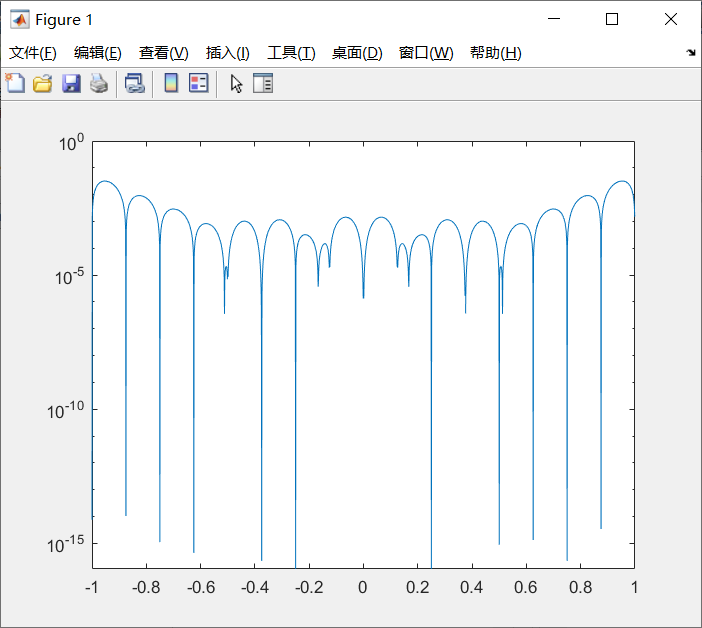
\includegraphics[width=0.8\textwidth]{3.png}
    	\caption{-1和1处一介二阶导数相等时插值逐点误差图像}\label{jpg:3}
	\end{figure}


	计算不同n值最大误差代码:\\
\begin{lstlisting}[frame=single,numbers=left]
clc,close
syms x;
left = -1;
right = 1;
n1 = 2000;
step1 = (right - left)/n1;
y = @(x) sin(4 * x.^2) + (sin(4 * x)).^2;
x1 = left:step1:right;

arr_n = [2.^4, 2.^5, 2.^6, 2.^7, 2.^8, 2.^9, 2.^10];
[~, ll] = size(arr_n);
maxn = zeros(1, ll);
figure
for j = 4 : 10
    n = 2.^j;
    step = (right - left)/n;
    x = left:step:right;
    res = myFunc(y, left, right, n);
    fy = zeros(1, n1 + 1);
    dev = zeros(1, n1 + 1);
    for i = 1 : n1
        seq = floor((x1(i) - left)/step) + 1;
        fy(i) = res(seq, 1) * x1(i).^3 + res(seq, 2)...
		 * x1(i).^2 + res(seq, 3) * x1(i) + res(seq, 4);
        dev(i) = abs(fy(i) - y(x1(i)));
    end
    maxn(j - 4 + 1) = max(dev(i));
end
loglog(arr_n, maxn)


function [res] = myFunc(y, left, right, n)
    sym y;
    step = (right - left)/n;
    lambda = 1/2;
    mu = 1 - lambda;
    d = zeros(n, 1);
    A = zeros(n, n);
    res = zeros(n, 4);
    para = left;
    for i = 2 : n
        para = para + step;
        d(i, 1) = 6 * (y(para + step) + y(para - step)...
		 - 2 * y(para)) / (2 * step.^2);
    end
    d(1, 1) = 6 / step * (y(left + step) - y(left)...
	 + y(right) - y(right - step)) / step;
    A(1, 1) =  4;
    A(1, 2) = 1;
    A(1, 3) = 1;
    for i = 2 : n - 1
        A(i, i - 1) = mu;
        A(i, i) = 2;
        A(i, i + 1) = lambda;
    end
    A(n, 1) = lambda;
    A(n, n - 1) = mu;
    A(n, n) = 2;
    m = A\d;
    m(n + 1, 1) = m(1, 1);
    para = left;
    for i = 1 : n
        para1 = para + step;
        A1 = [
            para.^3 para.^2 para 1;
            para1.^3 para1.^2 para1 1;
            6 * para 2 0 0;
            6 * para1 2 0 0;
            ];
        Y = [
            y(para);
            y(para1);
            m(i, 1);
            m(i + 1, 1);
            ];
        X = A1\Y;
        for j = 1 : 4
            res(i, j) = X(j, 1);
        end
        para = para1;
    end
end
\end{lstlisting}

	得到的最大误差如下图\ref{jpg:4}\\
	\begin{figure}[H]
		\centering
     	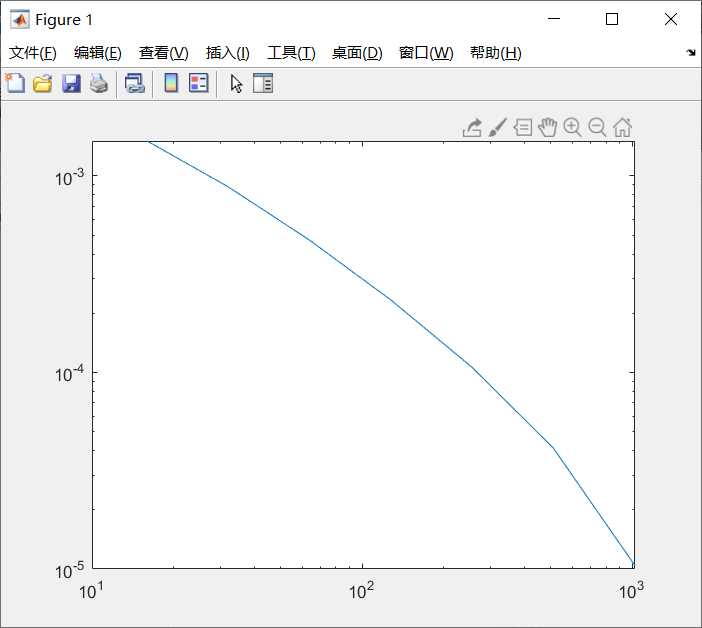
\includegraphics[width=0.8\textwidth]{4.png}
    	\caption{-1和1处一介二阶导数相等时不同n值最大误差图像}\label{jpg:4}
	\end{figure}

	\item[第二题]
	本题深入讨论Newton插值公式的性质。

	(a) (15分)对于一个光滑函数f(x),证明若$\{i_0, i_1, \dots, i_k\}$是$\{0, 1, \dots k\}$的任意一个排列,则
	$$
		f[x_0,x_1,\dots,x_k]=f[x_{i_0},x_{i_1},\dots,x_{i_k}]
	$$

	考虑证明
	$$
		f[x_0,x_1,\dots,x_k] = \sum_{i=0}^k {\frac {1} {\prod_{j = 0,j\ne i}^k {(x_i-x_j)}} f(x_i)}
	$$

	使用数学归纳法,当k = 1时
	$$
	f[x_0,x_1] = \frac {f(x_0)}{x_0-x_1}+\frac {f(x_1)} {x_1-x_0}
	$$
	显然成立

	当k ≥ 2时,假设n = k时结论成立,则n = k + 1时,有
	$$
	\begin{aligned}
		f[x_0,x_1,\dots,x_k,x_{k+1}] &=\frac {f[x_1,x_2,\dots,x_{k+1}]-f[x_0,x_1,\dots,x_k]}{x_{k+1}-x_0}\\
		&=\frac{\sum_{i=1}^{k+1} {\frac {1} {\prod_{j = 1,j\ne i}^{k+1} {(x_i-x_j)}} f(x_i)}-\sum_{i=0}^k {\frac {1} {\prod_{j = 0,j\ne i}^k {(x_i-x_j)}} f(x_i)}}{x_{k+1}-x_0}\\
		&=\sum_{i=0}^{k+1} {\frac{(x_i-x_0)-(x_i-x_{k+1})} {\prod_{j = 1,j\ne i}^{k+1} {(x_i-x_j)}} \frac {f(x_i)}{x_{k+1}-x_0}}\\
		&=	\sum_{i=0}^{k+1} {\frac {1} {\prod_{j = 0,j\ne i}^{k+1} {(x_i-x_j)}} f(x_i)}
	\end{aligned}
	$$
	等式成立,则等式得证,由此显然(a)中等式成立、、

	(b)(10分)课堂上我们提到了Chebyshev点
    $$ x_{j}=\cos (j \pi / n) \quad j=0,1, \ldots, n$$
    以及使用Chebyshev点可以有效地克服Runge现象。写一个MATLAB程序,令 $n=2^{2}, 2^{3}, 2^{4}, \ldots, 2^{7}$, 按照从右到左的顺序(即 $j$ 从小到大的顺序)使用对应的 $n+1$ 个Chebyshev点对定义在 $[-1,1]$ 上的Runge函数$$ f(x)=\frac{1}{1+25 x^{2}}$$进行插值,并取2000个等距点上的误差的最大值,用semilogy图描述插值区间上最大误差值随 $n$ 变化的情况(即横轴是 $n$)。\\
	
	代码如下:\\

\begin{lstlisting}[frame=single,numbers=left]
clc,close
syms x;
left = -1;
right = 1;
n1 = 2000;
m0 = 0;
mn = 0;
step1 = (right - left)/n1;
y = @(x) 1 / (1 + 25 * x.^2);
x1 = left:step1:right;

arr_n = [2.^2, 2.^3, 2.^4, 2.^5, 2.^6, 2.^7];
[~, ll] = size(arr_n);
maxn = zeros(1, ll);
for j = 2:7
    n = 2.^j;
    step = (right - left)/n;
    [Nx, fx] = newton(y, n, x1);
    maxn(j - 2 + 1) = max(abs(fx - Nx));
end
figure
%semilogy(x1, dev);
semilogy(arr_n, maxn)


function [Nx, fx] = newton(y, n, x1)
    sym y;  
    sym t;
    sym qb;
    syms x;
    qb = @(x) cos((x - 1) * pi / n);
    g = zeros(1, n + 1);
    for i = 1 : n + 1
        g(i) = y(qb(i));
    end
    for i = 2 : n + 1
        for j = n + 1 : -1 : i
            g(j) = (g(j) - g(j - 1))/...
			(qb(j) - qb(j - i + 1));
        end
    end
    [~, n1] = size(x1);
    t = ones(1, n1);
    Nx = zeros(1, n1);
    fx = zeros(1, n1);
    for i = 1 : n1        
        Nx(i) = y(qb(1));
        fx(i) = y(x1(i));
    end
    for i = 1 : n
        for j = 1 : n1
            t(j) = t(j) * (x1(j) - qb(i));
        end
        Nx = Nx + t * g(i + 1);
    end
end
\end{lstlisting}

	得到的最大误差如下图\ref{jpg:5}\\
	\begin{figure}[H]
		\centering
     	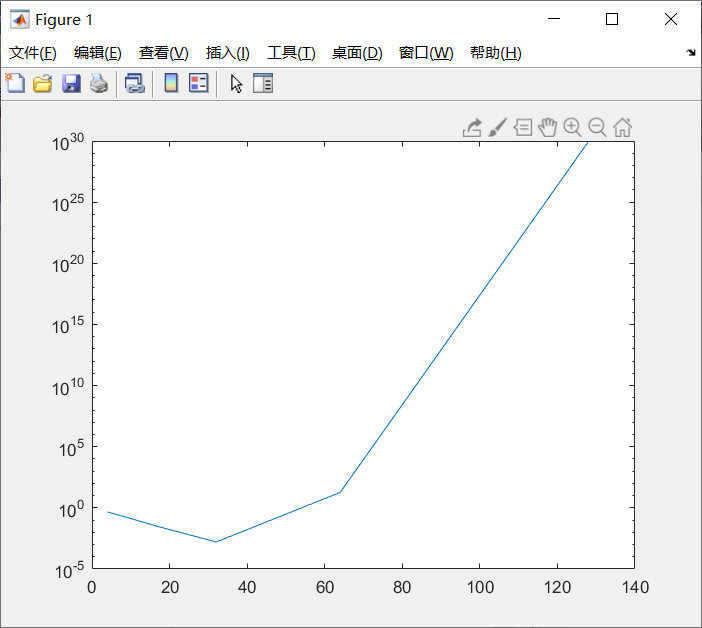
\includegraphics[width=0.8\textwidth]{5.png}
    	\caption{用切比雪夫点进行牛顿插值不同n值的最大误差图像}\label{jpg:5}
	\end{figure}
	
	(c)(10分) 重复上一问,但使用随机数种子rng(22)和randperm函数来随机计算 差商时插值点的使用顺序,取关于不同 $n$ 的2000个等距点上的误差的最大值,用semilogy图描述插值区间上最大误差值随 $n$ 变化的情况(即横轴是 $n$) 。\\

	代码如下:\\
\begin{lstlisting}[frame=single,numbers=left]
clc,close
syms x;
left = -1;
right = 1;
n1 = 2000;
m0 = 0;
mn = 0;
step1 = (right - left)/n1;
y = @(x) 1 / (1 + 25 * x.^2);
x1 = left:step1:right;

arr_n = [2.^2, 2.^3, 2.^4, 2.^5, 2.^6, 2.^7];
[~, ll] = size(arr_n);
maxn = zeros(1, ll);
for j = 2:7
    n = 2.^j;
    step = (right - left)/n;
    [Nx, fx] = newton(y, n, x1);
    maxn(j - 2 + 1) = max(abs(fx - Nx));
end
figure
%semilogy(x1, dev);
semilogy(arr_n, maxn)


function [Nx, fx] = newton(y, n, x1)
    sym y;  
    sym t;
    sym qb;
    syms x;
    rng(22);
    r = randperm(n + 1);
    qb = @(x) cos((r(x) - 1) * pi / n);
    g = zeros(1, n + 1);
    for i = 1 : n + 1
        g(i) = y(qb(i));
    end
    for i = 2 : n + 1
        for j = n + 1 : -1 : i
            g(j) = (g(j) - g(j - 1))/...
			(qb(j) - qb(j - i + 1));
        end
    end
    [~, n1] = size(x1);
    t = ones(1, n1);
    Nx = zeros(1, n1);
    fx = zeros(1, n1);
    for i = 1 : n1        
        Nx(i) = y(qb(1));
        fx(i) = y(x1(i));
    end
    for i = 1 : n
        for j = 1 : n1
            t(j) = t(j) * (x1(j) - qb(i));
        end
        Nx = Nx + t * g(i + 1);
    end
end
\end{lstlisting}	

	得到的最大误差如下图\ref{jpg:6}\\
	\begin{figure}[H]
		\centering
     	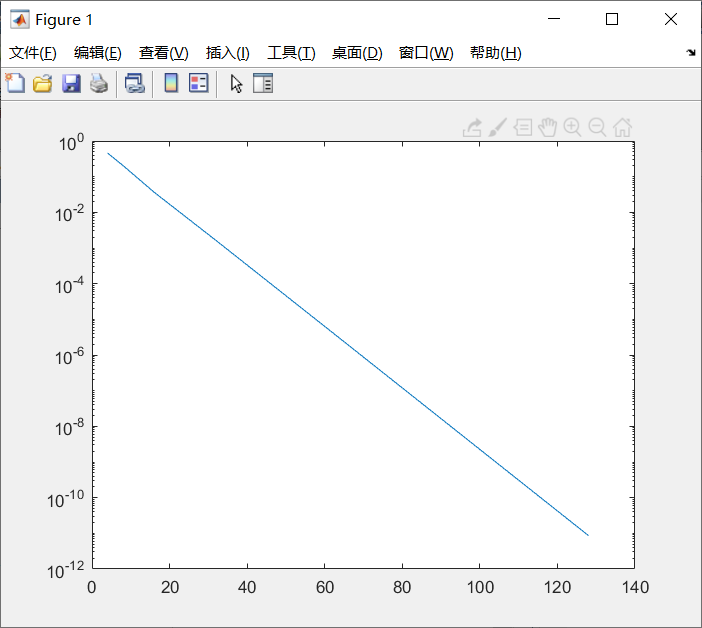
\includegraphics[width=0.8\textwidth]{6.png}
    	\caption{用随机切比雪夫点进行牛顿插值不同n值的最大误差图像}\label{jpg:6}
	\end{figure}

	\item[第三题] 
	本题用于讨论周期函数的Lagrange插值方法。对于周期函数而言,多项式不再是最有效的基函数,而等距插值点也不再会出现Runge现象。逼近周期函数的基函数通常选用三角函数或者复指数。同时注意对于周期函数而言,插值点数量和子区间个数相等。
	
	(a)(10分)在[0, 1]上关于周期函数的基于等间距插值点$x_j=\frac{j}{n},j=0,1,\dots,n-1$的Lagrange插值基函数为
                    $$
                        \ell_{k}(x)=\left\{\begin{array}{ll}
                            \frac{(-1)^{k}}{n} \sin (n \pi x) \csc \left(\pi\left(x-x_{k}\right)\right) & \text { 若 } n \text { 为奇数 } \\
                            \frac{(-1)^{k}}{n} \sin (n \pi x) \cot \left(\pi\left(x-x_{k}\right)\right) & \text { 若 } n \text { 为偶数 }
                        \end{array}\right.
                    $$
	证明对于n分别为奇数和偶数的情况下
                    $$
                        \ell_{k}\left(x_{j}\right)=\left\{\begin{array}{ll}
                            1 & k=j      \\
                            0 & k \neq j
                        \end{array}\right.
                    $$

	当n为奇数时,带入$x_j=\frac{j}{n}$有
	$$\ell_k(x_j)=\frac{(-1)^k}{n} \frac{\sin(j \pi)} {\sin(\frac {(j-k)\pi}{n})}$$
	当$k=j$时,$\sin (j\pi)=0,\sin(\frac {(j-k)n}{\pi})=0$,则
	$$
	\begin{aligned}
	\ell_k(x_j)&=\lim_{j \to k}\frac{(-1)^k}{n} \frac{\sin (j \pi)} {\sin(\frac {(j-k)\pi}{n})}\\
	&=\lim_{j \to k}\frac{(-1)^k}{n} \frac{\pi \cos(j\pi)} {\frac{\pi}{n}\cos(\frac {(j-k)\pi}{n})}\\
	&=\frac{(-1)^k}{n}\frac{\pi \cos(k\pi)}{\frac{\pi}{n}\cos(0)}\\
	&=1
	\end{aligned}
	$$
	当$k\ne j$时,$\sin (j\pi)=0,\sin(\frac {(j-k)n}{\pi})\ne 0$,则
	$$\ell_k(x_j)=0$$

	
	当n为偶数时,带入$x_j=\frac{j}{n}$有
	$$
	\begin{aligned}
	\ell_k(x_j)&=\frac{(-1)^k}{n} \frac{\sin(j \pi)} {\tan(\frac {(j-k)\pi}{n})}\\
	&=\frac{(-1)^k}{n} \frac{\sin(j \pi)} {\sin(\frac {(j-k)\pi}{n})} \cos(\frac {(j-k)\pi}{n})
	\end{aligned}
	$$
	而$k=j$时,$$\cos(\frac {(j-k)\pi}{n}=1$$
	故$$\ell_k(x_j)=\frac{(-1)^k}{n} \frac{\sin(j \pi)} {\sin(\frac {(j-k)\pi}{n})} \cos(\frac {(j-k)\pi}{n})=1*1=1$$
	$k\ne j$时,$$\cos(\frac {(j-k)\pi}{n}\leq 1$$
	故$$\ell_k(x_j)=\frac{(-1)^k}{n} \frac{\sin(j \pi)} {\sin(\frac {(j-k)\pi}{n})} \cos(\frac {(j-k)\pi}{n})=0*\cos(\frac {(j-k)\pi}{n})=0$$
	综上得证\\

	(b) (10分)用上述对应于$n$为偶数的Lagrange基函数构造Lagrange插值多项式,并用$n = 26$个点对周期函数$f(x)= \sin(2\pi x) e^{\cos(2\pi x)}$在$[0, 1]$上进行插值。取1000个等距点上的误差,用semilogy图描述插值区间上误差值随x变化的情况(即横轴是x)。\\

	代码如下:\\
\begin{lstlisting}[frame=single,numbers=left]
clc,close
n = 2^6;
n1 = 1000;
left = 0;
right = 1;
lx = @(x, k) (-1)^k / n * sin(n * pi * x) *...
 cot(pi * (x - k / n));
y = @(x) sin(2 * pi * x) * exp(cos(2 * pi * x));

x0 = left:(right - left) / n:right;
x1 = left:(right - left) / n1:right;
fx = zeros(1, n1 + 1);
px = zeros(1, n1 + 1);
yx = zeros(1, n + 1);
for i = 1 : n + 1
    yx(i) = y(x0(i));
end
for i = 1 : n1 + 1
    fx(i) = y(x1(i));
    para = x1(i);
    for j = 0 : n - 1
        px(i) = px(i) +  lx(para, j) * yx(j + 1);
    end
end

err = abs(fx - px);
figure
semilogy(x1, err);

\end{lstlisting}

得到的逐点误差如下图\ref{jpg:7}\\
	\begin{figure}[H]
		\centering
     	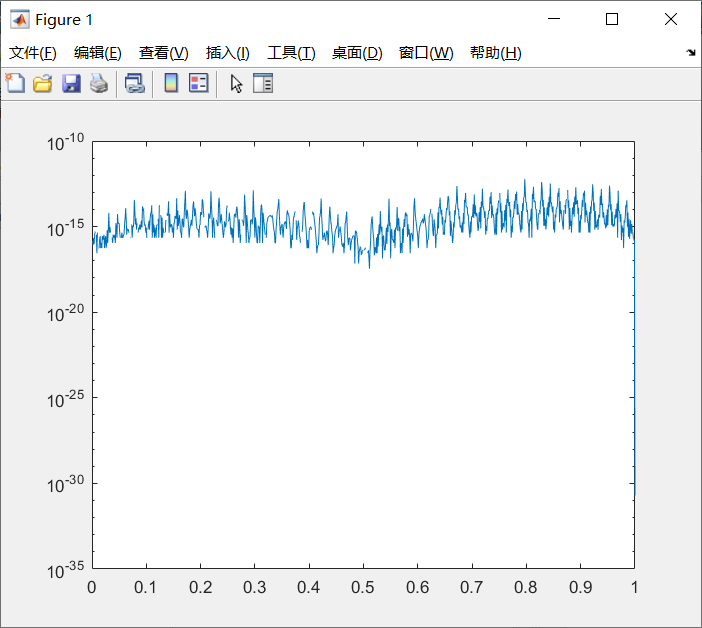
\includegraphics[width=0.8\textwidth]{7.png}
    	\caption{用拉格朗日插值的逐点图像}\label{jpg:7}
	\end{figure}

	\item[第四题]
(10分) 写程序完成课本59页第7题,并计算出你的拟合函数对比所给数据点的误差的2-范数。\\

	代码如下:\\
\begin{lstlisting}[frame=single,numbers=left]clc,close
x = [2.1, 2.5, 2.8, 3.2];
y = [.6087, .6849, .7368, .8111];

a1 = 0;
a2 = 0;
a3 = 0;
a4 = 0;
b1 = 0;
b2 = 0;
for i = 1 : 4
    a1 = a1 + y(i)^2;
    a2 = a2 + x(i) * y(i)^2;
    a3 = a2;
    a4 = a4 + x(i)^2 * y(i)^2;
    b1 = b1 + x(i) * y(i);
    b2 = b2 + x(i)^2 * y(i);
end

res = [a1 a2; a3 a4;]\[b1; b2;];
fx = zeros(1, 4);
for i = 1 : 4
    fx(i) = x(i)/ (res(1, 1) + res(2, 1) * x(i));
end

norm(fx - y, 2)
\end{lstlisting}

	运行得误差的2-范数为$$norm(fx-y,2)=0.005714477055041$$
\end{enumerate}
\end{document}